\begin{figure}[H]
\centering
\begin{subfigure}[H]{0.4\textwidth}
	\centering

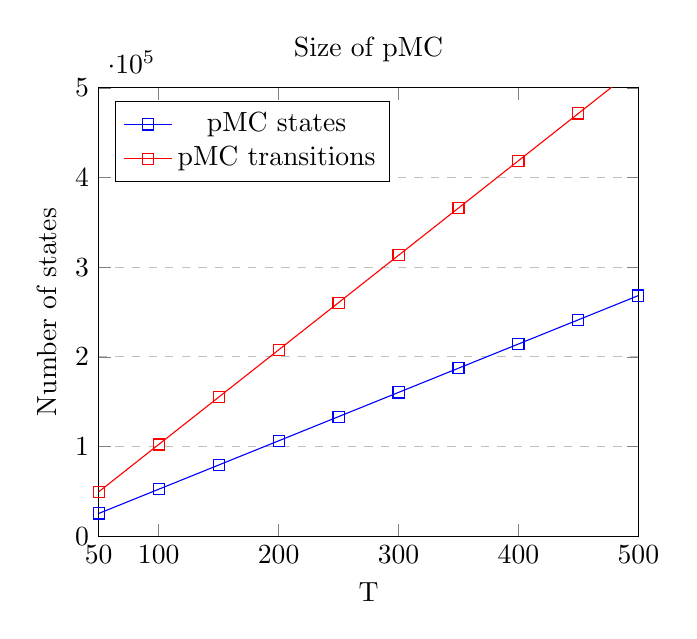
\begin{tikzpicture}
\begin{axis}[
    title={Size of pMC},
    xlabel={T},
    ylabel={Number of states},
    xmin=50, xmax=500,
    ymin=0, ymax=500000,
    xtick={50,100,200,300,400,500},
    ytick={0,100000,200000,300000,400000,500000},
    legend pos=north west,
    ymajorgrids=true,
    grid style=dashed,
]

\addplot[
    color=blue,
    mark=square,
    ]
    coordinates {
(50,25344)(100,52344)(150,79344)(200,106344)(250,133344)(300,160344)(350,187344)(400,214344)(450,241344)(500,268344)
    };
    
\addplot[
    color=red,
    mark=square,
    ]
    coordinates {
(50,49496)(100,102246)(150,154996)(200,207746)(250,260496)(300,313246)(350,365996)(400,418746)(450,471496)(500,524246)
    };
    \legend{pMC states, pMC transitions}

\end{axis}
\end{tikzpicture}
\end{subfigure}
\hfill
\begin{subfigure}[H]{0.4\textwidth}
	\centering
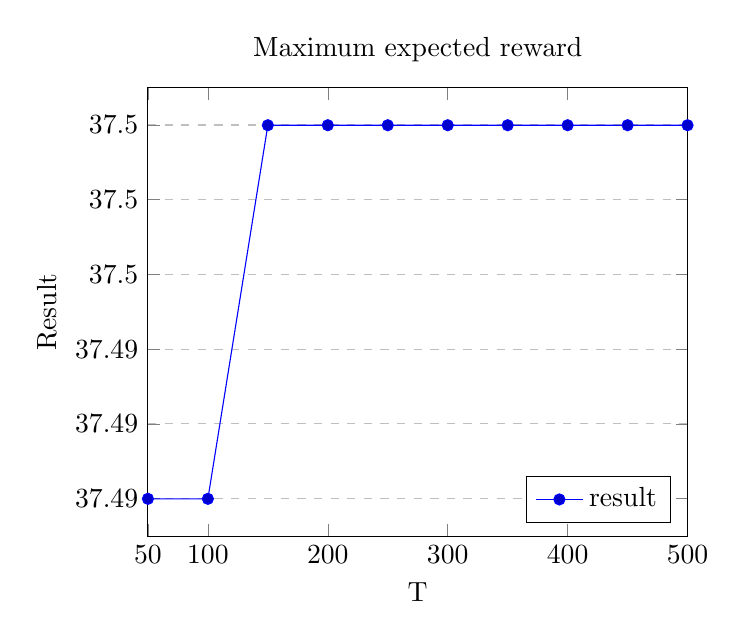
\begin{tikzpicture}

\begin{axis}[
    title={Maximum expected reward},
    xlabel={T},
    ylabel={Result},
    xmin=50, xmax=500,
    xtick={50,100,200,300,400,500},
    legend pos=south east,
    ymajorgrids=true,
    grid style=dashed]    
\addplot
    coordinates {
(50,37.49)(100,37.49)(150,37.5)(200,37.5)(250,37.5)(300,37.5)(350,37.5)(400,37.5)(450,37.5)(500,37.5)
    };
    \legend{result}
    
\end{axis}
\end{tikzpicture}
\end{subfigure}

\begin{subfigure}[H]{0.4\textwidth}
	\centering
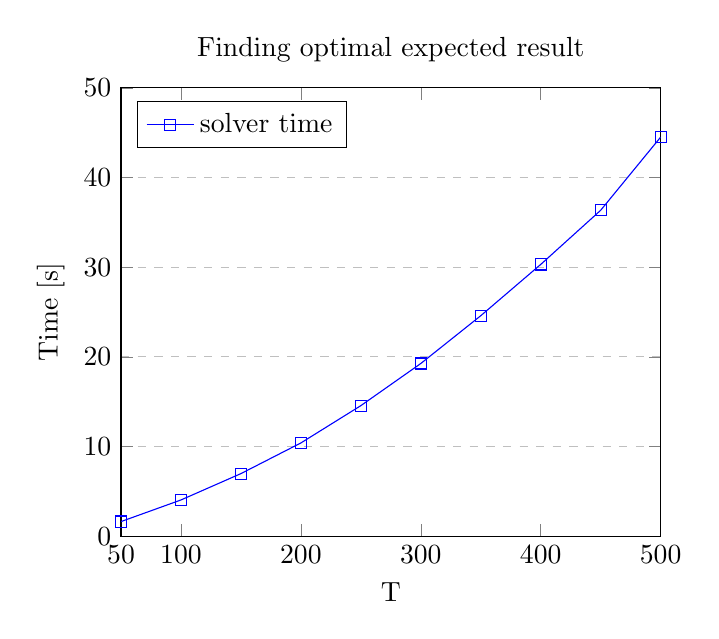
\begin{tikzpicture}
\begin{axis}[
    title={Finding optimal expected result},
    xlabel={T},
    ylabel={Time [s]},
    xmin=50, xmax=500,
    ymin=0, ymax=50,
    xtick={50,100,200,300,400,500},
    ytick={0,10,20,30,40,50},
    legend pos=north west,
    ymajorgrids=true,
    grid style=dashed,
]

\addplot[
    color=blue,
    mark=square,
    ]
    coordinates {
(50,1.63)(100,4.04)(150,6.98)(200,10.40)(250,14.56)(300,19.26)(350,24.59)(400,30.31)(450,36.35)(500,44.51)
    };
    \legend{solver time}

\end{axis}
\end{tikzpicture}
\end{subfigure}
\hfill
\begin{subfigure}[H]{0.4\textwidth}
	\centering
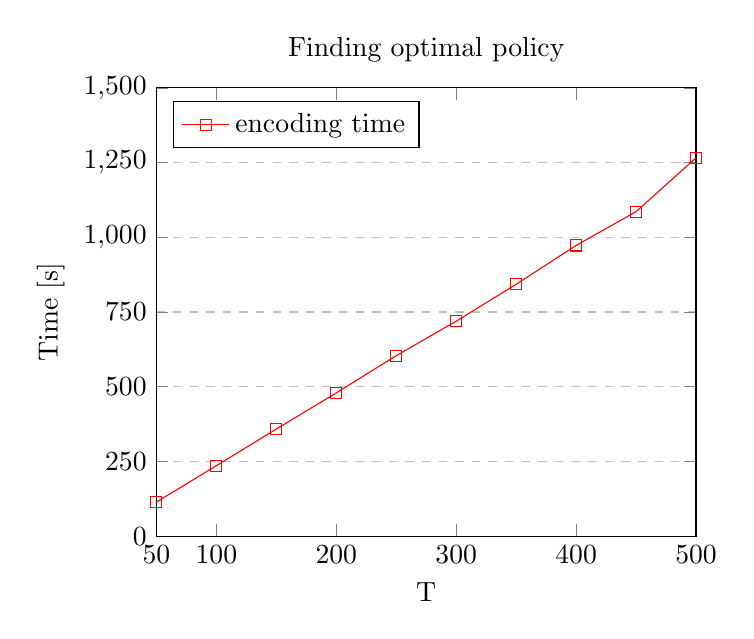
\begin{tikzpicture}
\begin{axis}[
    title={Finding optimal policy},
    xlabel={T},
    ylabel={Time [s]},
    xmin=50, xmax=500,
    ymin=0, ymax=1500,
    xtick={50,100,200,300,400,500},
    ytick={0,250,500,750,1000,1250,1500},
    legend pos=north west,
    ymajorgrids=true,
    grid style=dashed,
]
    
\addplot[
    color=red,
    mark=square,
    ]
    coordinates {
(50,114.17)(100,235.75)(150,358.44)(200,479.33)(250,603.95)(300,719.27)(350,842.76)(400,972.81)(450,1085.68)(500,1265.92)
    };
    \legend{encoding time}
    
\end{axis}
\end{tikzpicture}
\end{subfigure}
\caption{Results for $N=5$}
\end{figure}









\begin{figure}[H]
\centering
\begin{subfigure}[H]{0.4\textwidth}
	\centering

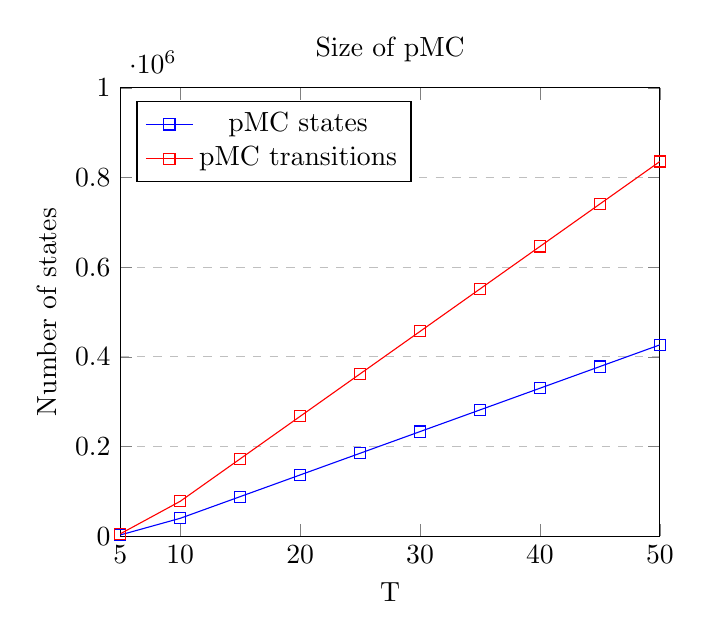
\begin{tikzpicture}
\begin{axis}[
    title={Size of pMC},
    xlabel={T},
    ylabel={Number of states},
    xmin=5, xmax=50,
    ymin=0, ymax=1000000,
    xtick={5,10,20,30,40,50},
    ytick={0,200000,400000,600000,800000,1000000},
    legend pos=north west,
    ymajorgrids=true,
    grid style=dashed,
]

\addplot[
    color=blue,
    mark=square,
    ]
    coordinates {
(5,2740)(10,39908)(15,88268)(20,136628)(25,184988)(30,233348)(35,281708)(40,330068)(45,378428)(50,426788)
    };
    
\addplot[
    color=red,
    mark=square,
    ]
    coordinates {
(5,5223)(10,77819)(15,172564)(20,267309)(25,362054)(30,456799)(35,551544)(40,646289)(45,741034)(50,835779)
    };
    \legend{pMC states, pMC transitions}
    
\end{axis}
\end{tikzpicture}
\end{subfigure}
\hfill
\begin{subfigure}[H]{0.4\textwidth}
	\centering
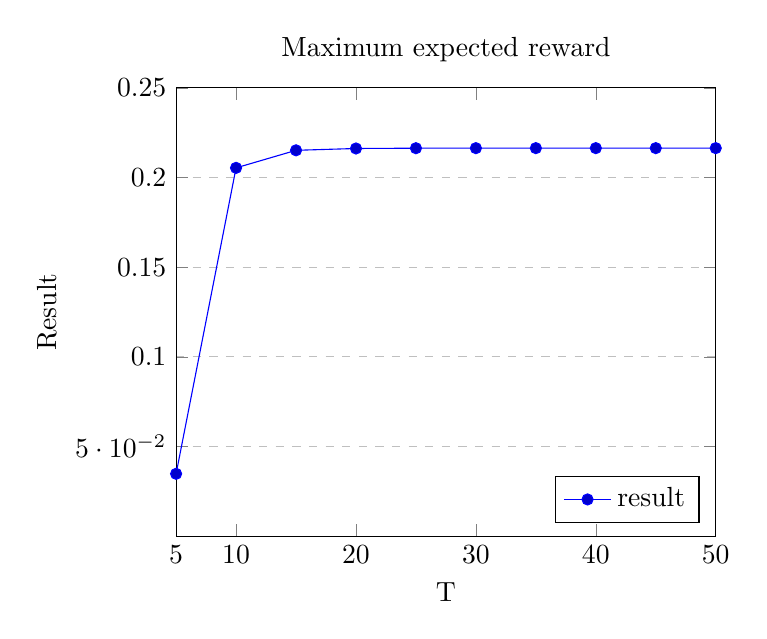
\begin{tikzpicture}

\begin{axis}[
    title={Maximum expected reward},
    xlabel={T},
    ylabel={Result},
    xmin=5, xmax=50,
    ymin=0, ymax=0.25,
    xtick={5,10,20,30,40,50},
    ytick={0.05,0.1,0.15,0.2,0.25},
    legend pos=south east,
    ymajorgrids=true,
    grid style=dashed,
]
    
\addplot
    coordinates {
(5,0.034790)(10,0.20539)(15,0.21518)(20,0.21620)(25,0.21636)(30,0.21639)(35,0.21640)(40,0.21640)(45,0.21640)(50,0.21640)
    };
    \legend{result}
    
\end{axis}
\end{tikzpicture}
\end{subfigure}

\begin{subfigure}[H]{0.4\textwidth}
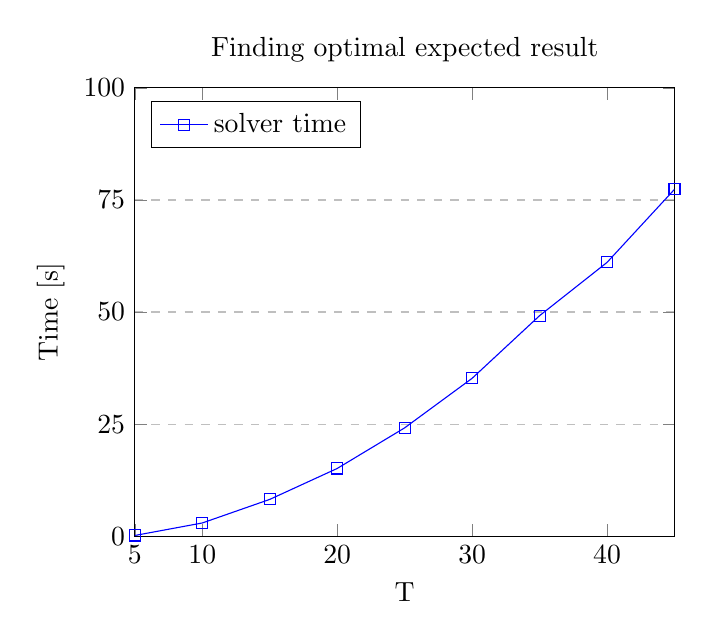
\begin{tikzpicture}
\begin{axis}[
	title={Finding optimal expected result},
    xlabel={T},
    ylabel={Time [s]},
    xmin=5, xmax=45,
    ymin=0, ymax=100,
    xtick={5,10,20,30,40,50},
    ytick={0,25,50,75,100},
    legend pos=north west,
    ymajorgrids=true,
    grid style=dashed,
]

\addplot[
    color=blue,
    mark=square,
    ]
    coordinates {
(5,0.16)(10,2.95)(15,8.21)(20,15.11)(25,24.17)(30,35.22)(35,49.19)(40,61.07)(45,77.37)
    };
    \legend{solver time}
    
\end{axis}
\end{tikzpicture}
\end{subfigure}
\hfill
\begin{subfigure}[H]{0.4\textwidth}
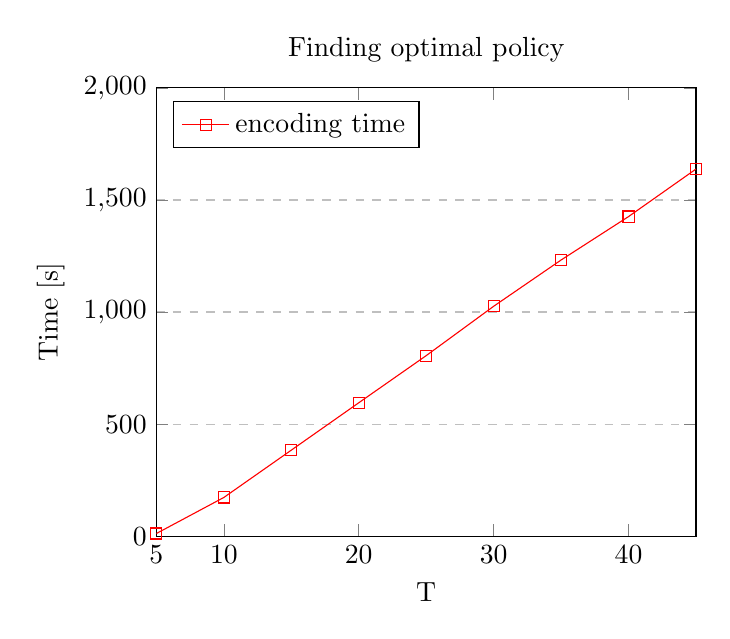
\begin{tikzpicture}
\begin{axis}[
title={Finding optimal policy},
    xlabel={T},
    ylabel={Time [s]},
    xmin=5, xmax=45,
    ymin=0, ymax=2000,
    xtick={5,10,20,30,40,50},
    ytick={0,500,1000,1500,2000},
    legend pos=north west,
    ymajorgrids=true,
    grid style=dashed,
]
    
\addplot[
    color=red,
    mark=square,
    ]
    coordinates {
(5,11.95)(10,172.79)(15,383.88)(20,595.19)(25,805.52)(30,1025.71)(35,1232.19)(40,1425.90)(45,1638.00)
    };
    \legend{encoding time}
    
\end{axis}
\end{tikzpicture}
\end{subfigure}
\caption{Results for $N=10$}
\end{figure}